\documentclass{article}
% Required package
\usepackage{amsmath}
\usepackage{arxiv}

\usepackage[utf8]{inputenc}
\usepackage[english, russian]{babel}
\usepackage[T1]{fontenc}
\usepackage{url}
\usepackage{booktabs}
\usepackage{algorithm}
\usepackage{algpseudocode}
\usepackage{amsfonts}
\usepackage{nicefrac}
\usepackage{microtype}
\usepackage{lipsum}
\usepackage{graphicx}
\usepackage{natbib}
\usepackage{doi}



\title{Создание персонализированных генераций изображений}

\author{ Кристина М.~Казистова \\
	ФПМИ\\
	МФТИ\\
	Долгопрудный \\
	\texttt{kazistova.km@phystech.edu} \\
	%% examples of more authors
	\And
	Степанов Илья Дмитриевич \\
	ФПМИ\\
	МФТИ\\
	Долгопрудный \\
	\texttt{iliatut94@gmail.com} \\
    \And
	Филатов Андрей Викторович \\
	Сколковский Институт Технологий\\
	Москва \\
	\texttt{filatovandreiv@gmail.com} \\
	%% \AND
	%% Coauthor \\
	%% Affiliation \\
	%% Address \\
	%% \texttt{email} \\
	%% \And
	%% Coauthor \\
	%% Affiliation \\
	%% Address \\
	%% \texttt{email} \\
	%% \And
	%% Coauthor \\
	%% Affiliation \\
	%% Address \\
	%% \texttt{email} \\
}
\date{}


\renewcommand{\undertitle}{}
\renewcommand{\headeright}{}
\renewcommand{\shorttitle}{\textit{Создание персонализированных генераций изображений}}

%%% Add PDF metadata to help others organize their library
%%% Once the PDF is generated, you can check the metadata with
%%% $ pdfinfo template.pdf

\begin{document}
\maketitle
    
\begin{abstract}
        Модели генерации изображений по тексту совершили значительный скачок в области искусственного интеллекта, обеспечив высококачественный и разнообразный синтез изображений из заданного текстового описания. Однако, когда возникает запрос на генерацию специфичного объекта, в нашем случае человека, модель не может сгенерировать его с необходимой точностью и передать его идентичность. Предлагается решение, которое будет способно генерировать изображения заданного человека в различных вариациях в высоком разрешении. Мы представляем подход, в основе которого лежит метод IP-Adapter. Данный подход способен обрабатывать несколько изображений одновременно, что приводит к повышению качества генерации.
\end{abstract}

\textbf{Ключевые слова}: Диффузионная модель, Stable Diffusion\cite{DBLP:journals/corr/abs-2112-10752}, IP-Adapter\cite{ye2023ip-adapter}, DreamBooth\cite{ruiz2022dreambooth}.

\section{Введение}В последние годы наблюдается быстрое развитие генеративных моделей, которые решают задачу генерации изображений по тексту. Существующие модели способны генерировать разнообразные изображения по текстовым описаниям с высокой точностью. Однако, в процессе работы с моделями генерации изображений возникают определенные проблемы, одной из которых является недостаточное соответствие сгенерированных изображений исходным текстовым описаниям. Наша задача заключается в повышении качества визуальных представлений за счет большего количества изображений. В работе рассматриваются методы, которые позволяют решить вышеупомянутые проблемы, и затем сравниваются между собой. Все описанные далее подходы основаны на применении диффузионной модели\cite{DBLP:journals/corr/abs-2112-10752}. 

Диффузионная модель состоит из двух процессов: прямого и обратного.Во время прямого процесса ко входным данным постепенно добавляется шум, а во время обратного процесса модель постепенно восстанавливает данные из шума. Эта модель позволяет создавать высококачественные изображения на основе текстовых и графических подсказок, открывая новые возможности в области синтеза изображений.

Первый представленный метод --- это DreamBooth\cite{ruiz2022dreambooth}.Он принимает на вход несколько изображений одного объекта вместе с соответствующим названием класса и возвращает специальный токен, идентифицирующий объект, который затем встраивается в текстовое описание, по которой генерируется желаемое изображение. Проблемы данного метода заключаются в слабой адаптивности, отсутствии обобщения и необходимости обучать всю диффузионную модель. 

Второй метод --- это IP-Adapter\cite{ye2023ip-adapter}. Он состоит из двух частей: энкодера для извлечения признаков изображения, текста и адаптированных модулей с механизмом перекрестного внимания\cite{DBLP:journals/corr/VaswaniSPUJGKP17}. Метод принимает на вход только одно изображение объекта. Однако одной картинки может быть мало, для того чтобы модель могла уловить все необходимые зависимости. 

В работе предлагается третий метод, представляющий собой модификацию IP-Adapter. На вход подаются несколько изображений вместо одного, причем каждому изображению соответствует своя текстовая подсказка. В процессе обучения модели одно изображение удаляется равновероятно, и модель учится восстанавливать это удаленное изображение, опираясь на текстовое описание и другие имеющиеся изображения.К векторным представлениям изображений применяется агрегирующая функция. За счет подачи нескольких изображений добиваемся лучшей передачи идентичности. 
Рассмотренные методы сравниваются между собой по метрикам качества генерации и разнообразия, метрикам идентичности.
Исследование проводится на выборке из датасета LFW Deep Funneled\cite{LFWTech} --- датасете изображений знаменитостей в высоком разрешении. 

\section{Постановка задачи}

Определим датасет как $ \mathfrak{D}=\{ ({x}_{i}, \mathbf{\tau}_{i}): i = 1, \dots, n\}$, ${x}_{i}$ --- изображение, $\mathbf{\tau}_{i}$ -- соответствующий текстовый промпт. Рассматривается модель $\epsilon_{\theta}$ из класса диффузионных моделей. На этапе обучения на каждом шаге из $\mathfrak{D}$ удаляется изображение ${x}_{j}, j \sim \mathcal{U}\{1, \dots, n\}$, и модель учится восстанавливать его по оставшимся изображениям.

Определим функцию потерь: 
\begin{equation}
\mathcal{L}(\epsilon, \epsilon_{\theta}) = \mathbb{E}_{\epsilon \sim N(0, I),\mathbf{c}_{\tau}, \mathbf{c}_{i}, t, \mathbf{c}^{j}_{t}} \|\epsilon - \epsilon_{\theta}(\mathbf{c}_{\tau}, \mathbf{c}_{i}, t, \mathbf{c}^{j}_{t})\|^2,
\end{equation}
где $\mathbf{c}_{\tau} = \Gamma_\tau(\tau_j)$ --- текстовые признаки удаленного изображения, полученные путем применения текстового энкодера $\Gamma_\tau$ к текстовому промпту $\tau_j$; $\mathbf{c}_{i} = G(\Gamma_i(x_1), \dots, \Gamma_i(x_{j-1}), \Gamma_i(x_{j+1}), \dots, \Gamma_i(x_n))$ --- признаки оставшихся изображений, являющиеся результатом применения агрегирующей функции $G$ к эмбеддингам изображений, полученным с помощью image-энкодера $\Gamma_i$; $\mathbf{c}^{j} = \Gamma_i(x_j)$ --- признаки удаленного изображения; $t \in [0, T]$ --- временной шаг диффузионного процесса, $\mathbf{c}^{j}_{t} = \alpha_t \mathbf{c}^{j}  + \sigma_t \epsilon$ --- зашумленные данные удаленного изображения на шаге $t$; $\alpha_t, \sigma_t$ --- предопределенные функции от $t$, определяющие диффузионный процесс.

Решается следующая оптимизационная задача:

\begin{equation}
\epsilon_{\theta}^* = \arg \min_{\epsilon_{\theta}}\mathcal{L}(\epsilon, \epsilon_{\theta}),
\end{equation}

Текстовые признаки, извлеченные из текстового энкодера, передаются в предобученную диффузионную модель через слои перекрестного внимания. Для передачи в модель признаков изображения каждому слою перекрестного внимания для текстовых признаков сопоставляется слой перекрестного внимания для признаков изображения. Выход полученного слоя изолированного перекрестного внимания определяется как:

\begin{equation}
\mathbf{Z}^{new} = Attention(\mathbf{Q}, \mathbf{K}, \mathbf{V}) + \lambda Attention(\mathbf{Q}, \mathbf{K}^{\prime}, \mathbf{V}^{\prime}), 
\end{equation}
где $\lambda$ --- весовой коэффициент, $\mathbf{Z}$ --- признаки запроса, $\mathbf{Q} = \mathbf{Z}\mathbf{W}_q$, $\mathbf{K} = \mathbf{c}_t\mathbf{W}_k, \mathbf{K}^{\prime} = \mathbf{c}_i {\mathbf{W}}^{\prime}_{k}, \mathbf{V} = \mathbf{c}_t\mathbf{W}_{v}, \mathbf{c}_i {\mathbf{W}}^{\prime}_{v}$ --- матрицы запросов, ключей и значений механизмов внимания для текста и изображений соответственно, a $\mathbf{W}_q, \mathbf{W}_k, {\mathbf{W}}^{\prime}_{k}, \mathbf{W}_v, {\mathbf{W}}^{\prime}_{v}, {\mathbf{W}}^{\prime}_k,{\mathbf{W}}^{\prime}_v$ --- соответствующие матрицы весов. 

Для определения качества модели введем метрики качества генерации Frechet Inception Distance (FID)\cite{DBLP:journals/corr/HeuselRUNKH17} и Inception Score (IS)\cite{DBLP:journals/corr/SalimansGZCRC16}: 

\begin{equation}
FID = ||\mu_p - \mu_q||^2 + Tr(\mathbf{\Sigma_p} + \mathbf{\Sigma_q} - 2(\mathbf{\Sigma_p}\mathbf{\Sigma_q})^{1/2})
\end{equation}

где \( \mu_p \) и \( \mu_q \) --- средние значения признаков в реальных и сгенерированных изображениях соответственно, \( \mathbf{\Sigma_p} \) и \( \mathbf{\Sigma_q} \) --- ковариационные матрицы для распределений признаков на реальных и сгенерированных изображениях соответственно.
\begin{equation}
IS(x) = \exp(\mathbb{E}_x \left[ D_{KL}(p(y | x) || p(y)) \right] )
\end{equation}

Где \( D_{KL} \) - дивергенция Кульбака-Лейблера для двух распределений; \(p(y|x)\) - вероятность класса \(y\) для изображения \(x\); \(p(y)\) - равномерное распределение на множестве классов.

\section{Метод}
В данной секции мы сначала введем необходимые понятия, затем опишем принцип работы существующих методов решения поставленной задачи: IP-Adapter и DreamBooth. Наконец, представим описание разработанного нами метода.
\subsection{Вводные сведения}
\subsubsection{Диффузионные модели}
Диффузионная модель состоит из двух процессов: прямого и обратного.

Прямой процесс представляет собой последовательность зашумленных версий входного изображения $x_0, \dots, x_T$, где $T$ --- количество шагов, a $x_t$ получается по следующей формуле: 
\begin{equation}
x_t = \sqrt{1-\beta_t}x_{t-1}+\sqrt{\beta_t}\varepsilon,
\end{equation}
где $\varepsilon \sim \mathcal{N}(0, I)$, 
\begin{equation}
x_t|x_{t-1} \sim \mathcal{N}(\sqrt{1-\beta_t}x_{t-1}, \beta_t I).
\end{equation}
При $T \rightarrow \infty, x_T \rightarrow \mathcal{N}(0, I).$ На последнем шаге итераций получается гауссовский шум. 

Положим $\alpha_t=1-\beta_t, \overline{\alpha_t} = \prod\limits_{s = 1}^t\alpha_s$. Тогда 
\begin{equation}
x_t = \sqrt{\overline{\alpha_t}}x_0+\sqrt{1-\overline{\alpha_t}}\varepsilon,
\end{equation}
где $\varepsilon \sim \mathcal{N}(0, I)$, 
\begin{equation}
x_t|x_0 \sim \mathcal{N}(\sqrt{\overline{\alpha_t}}x_0, (1-\overline{\alpha_t}) I).
\end{equation}

Во время обратного процесса исходное изображение восстанавливается из шума. Знаем $x_T\sim \mathcal{N}(0, I)$. Семплирование происходит итеративно шаг за шагом:
\begin{equation}
\hat{x}_{t-1} = \frac{1}{\sqrt{\alpha_t}}\left( \hat{x}_t - \frac{1-\alpha_t}{\sqrt{1-\overline{\alpha_t}}}\hat{\epsilon}_t\right) + \sqrt{\beta_t}\epsilon,
\end{equation}
где $\hat{x}_t$ --- восстановленное изображение на итерации $t$, при этом, если $t = T$, то $\hat{x}_t = x_t$; $\hat{\epsilon}_t$ --- реконструкция шума, полученная моделью для $\hat{x}_t$; $\epsilon \sim \mathcal{N}(0, I)$ --- шум, который позволяет генерировать различные изображения. 

\subsubsection{Stable Diffusion}
Процесс работы модели Stable Diffusion состоит из трех основных этапов. Сначала энкодер CLIP\cite{DBLP:journals/corr/abs-2103-00020} преобразует входное изображение в эмбеддинг в пространстве меньшей размерности. Затем диффузионная модель выполняет преобразование полученного эмбеддинга (в скрытом пространстве). Наконец, VAE\cite{DBLP:journals/corr/abs-1906-02691} декодер переводит преобразованный эмбеддинг в изображение исходного размера. В качестве диффузионной модели используется UNet\cite{DBLP:journals/corr/RonnebergerFB15} архитектура с механизмом внимания.

\subsubsection{Classifier-free Guidance}
Можно регулировать силу влияния условия $c$ без специального классификатора. Метод classifier-free guidance\cite{ho2022classifierfree} позволяет увеличить степень, с которой модель ориентируется на промпт. Во время семплирования предсказание получается путем линейной комбинации предсказаний обусловленной и необусловленной моделей: 
\begin{equation}
\hat{\epsilon}_{\theta}(x_t, c, t) = w\epsilon_{\theta}(x_t, c, t) + (1-w)\epsilon_{\theta}(x_t, t),
\end{equation}

где $w$ --- весовой коэффицент, $t \in [0, T]$ --- временной шаг диффузионного процесса, $x_t$ --- зашумленные данные удаленного изображения на шаге $t$.

\subsection{DreamBooth}

\begin{figure}[H]
    \centering
    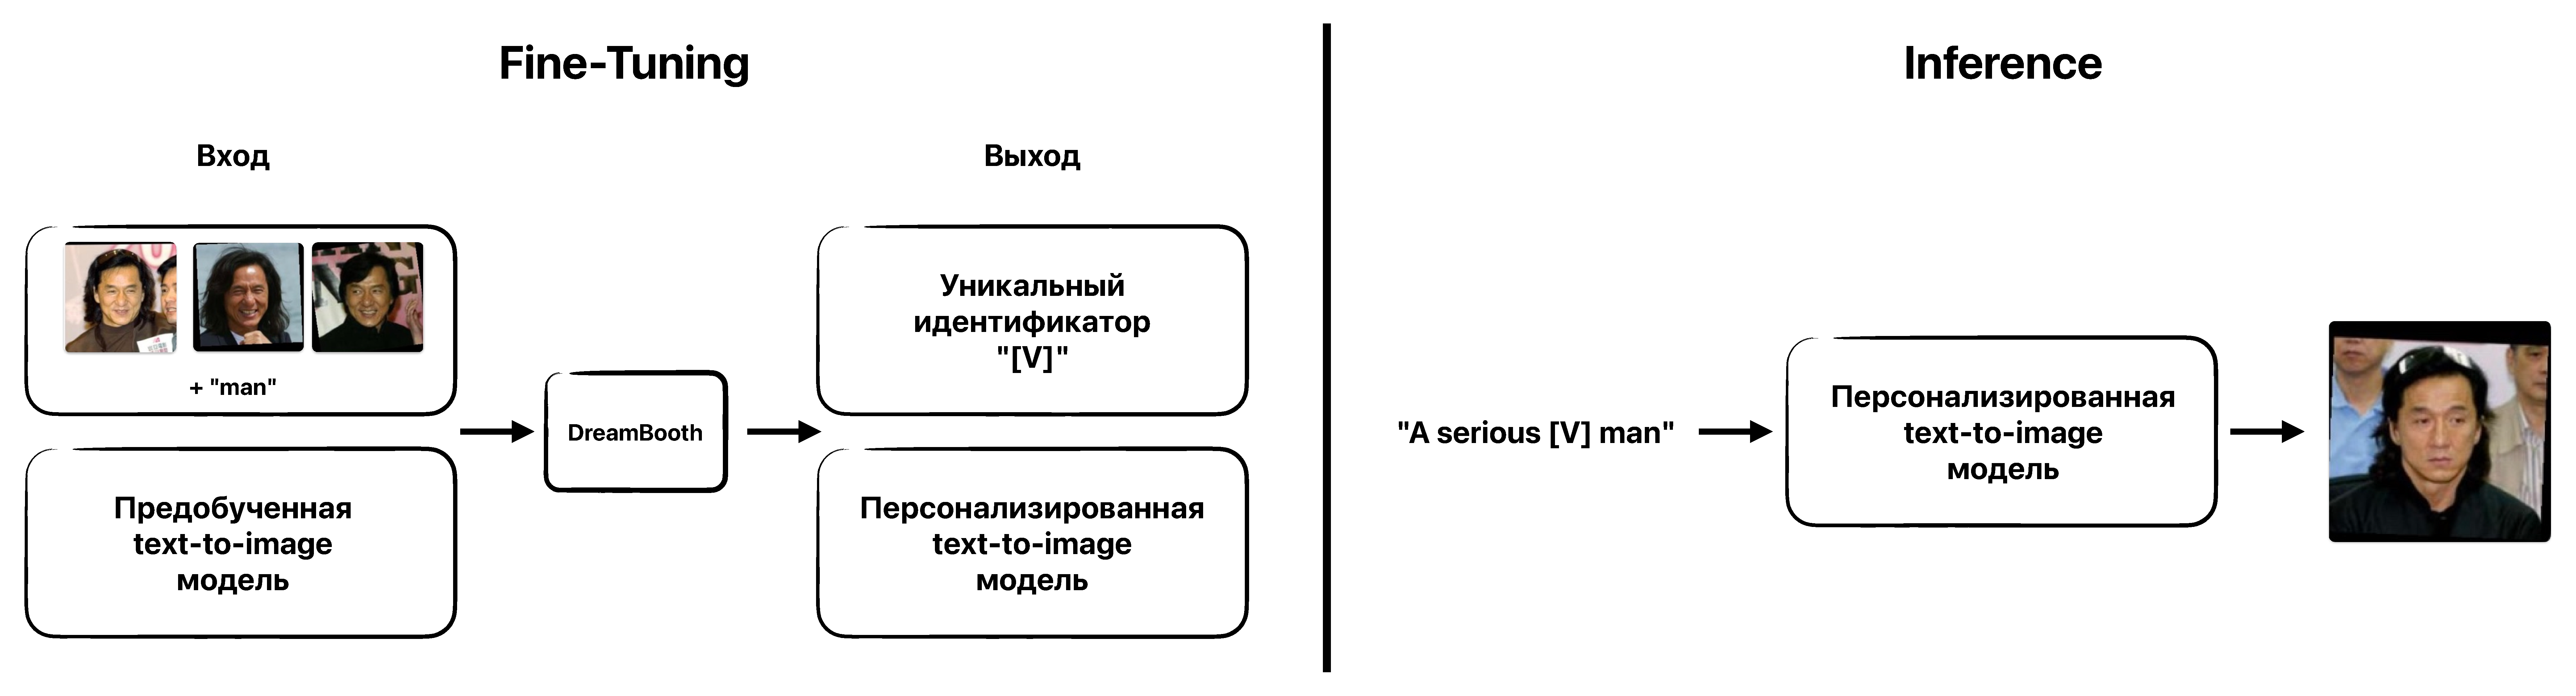
\includegraphics[width=1\textwidth]{dreambooth.pdf}
    \caption{DreamBooth}
    \label{fig:simple}
\end{figure}

В основе данной модели лежит предобученная диффузионная text-to-image модель $\hat{x}_{\theta}$, функция потерь которой определяется как:
\begin{equation}
\mathbb{E}_{\mathbf{x}, \epsilon \sim \mathca{N}(0, I), \mathbf{c}, t} w_t \|\hat{x}_{\theta}(\alpha_t \mathbf{x} + \sigma_t \epsilon, \mathbf{c}) - \mathbf{x}\|^2,
\end{equation}
где $\mathbf{x}$ --- латентное представление исходного изображения, $\mathbf{c} = \Gamma(P)$ --- вектор условия, полученный с помощью текстового энкодера $\Gamma$ и текстового промпта $P$, $t \in [0, T]$ обозначает временной шаг диффузионного процесса; $\alpha_t$, $\sigma_t$, $w_t$ --- предопределенные функции от $t$, определяющие процесс диффузии. 

Исходная диффузионная модель дообучается на нескольких входных изображениях одного объекта в паре с текстовым промптом, содержащим название класса, к которому принадлежит данный объект. Генерируются данные  $\mathbf{x_{pr}} = \hat{x}(z, \mathbf{c_{pr}})$ с использованием сэмплера на основе предобученной диффузионной модели со случайным начальным шумом $z \sim \mathcal{N}(0, I)$ и вектором условия $\mathbf{c_{pr}} := \Gamma(f("$a [class  noun$]"))$, где $f$ --- токенизатор. Функция потерь принимает следующий вид: 
\begin{equation}
\mathbb{E}_{\mathbf{x}, \epsilon, \epsilon^{\prime}, \mathbf{c}, t} [w_t \|\hat{x}_{\theta}(\alpha_t \mathbf{x} + \sigma_t \epsilon, \mathbf{c}) - \mathbf{x}\|^2 + \lambda w_{t^{\prime}} \|\hat{x}_{\theta}(\alpha_{t^{\prime}} \mathbf{x_{pr}} + \sigma_{t^{\prime}} \epsilon^{\prime}, \mathbf{c_{pr}}) - \mathbf{x_{pr}}\|^2],
\end{equation}
где $\lambda$ --- весовой коэффициент.

Генерация изображений происходит путем встраивания уникального идентификатора в текстовый промпт в виде: "a [identifier] [class noun]". 


\subsection{IP-Adapter}

\begin{figure}[H]
    \centering
    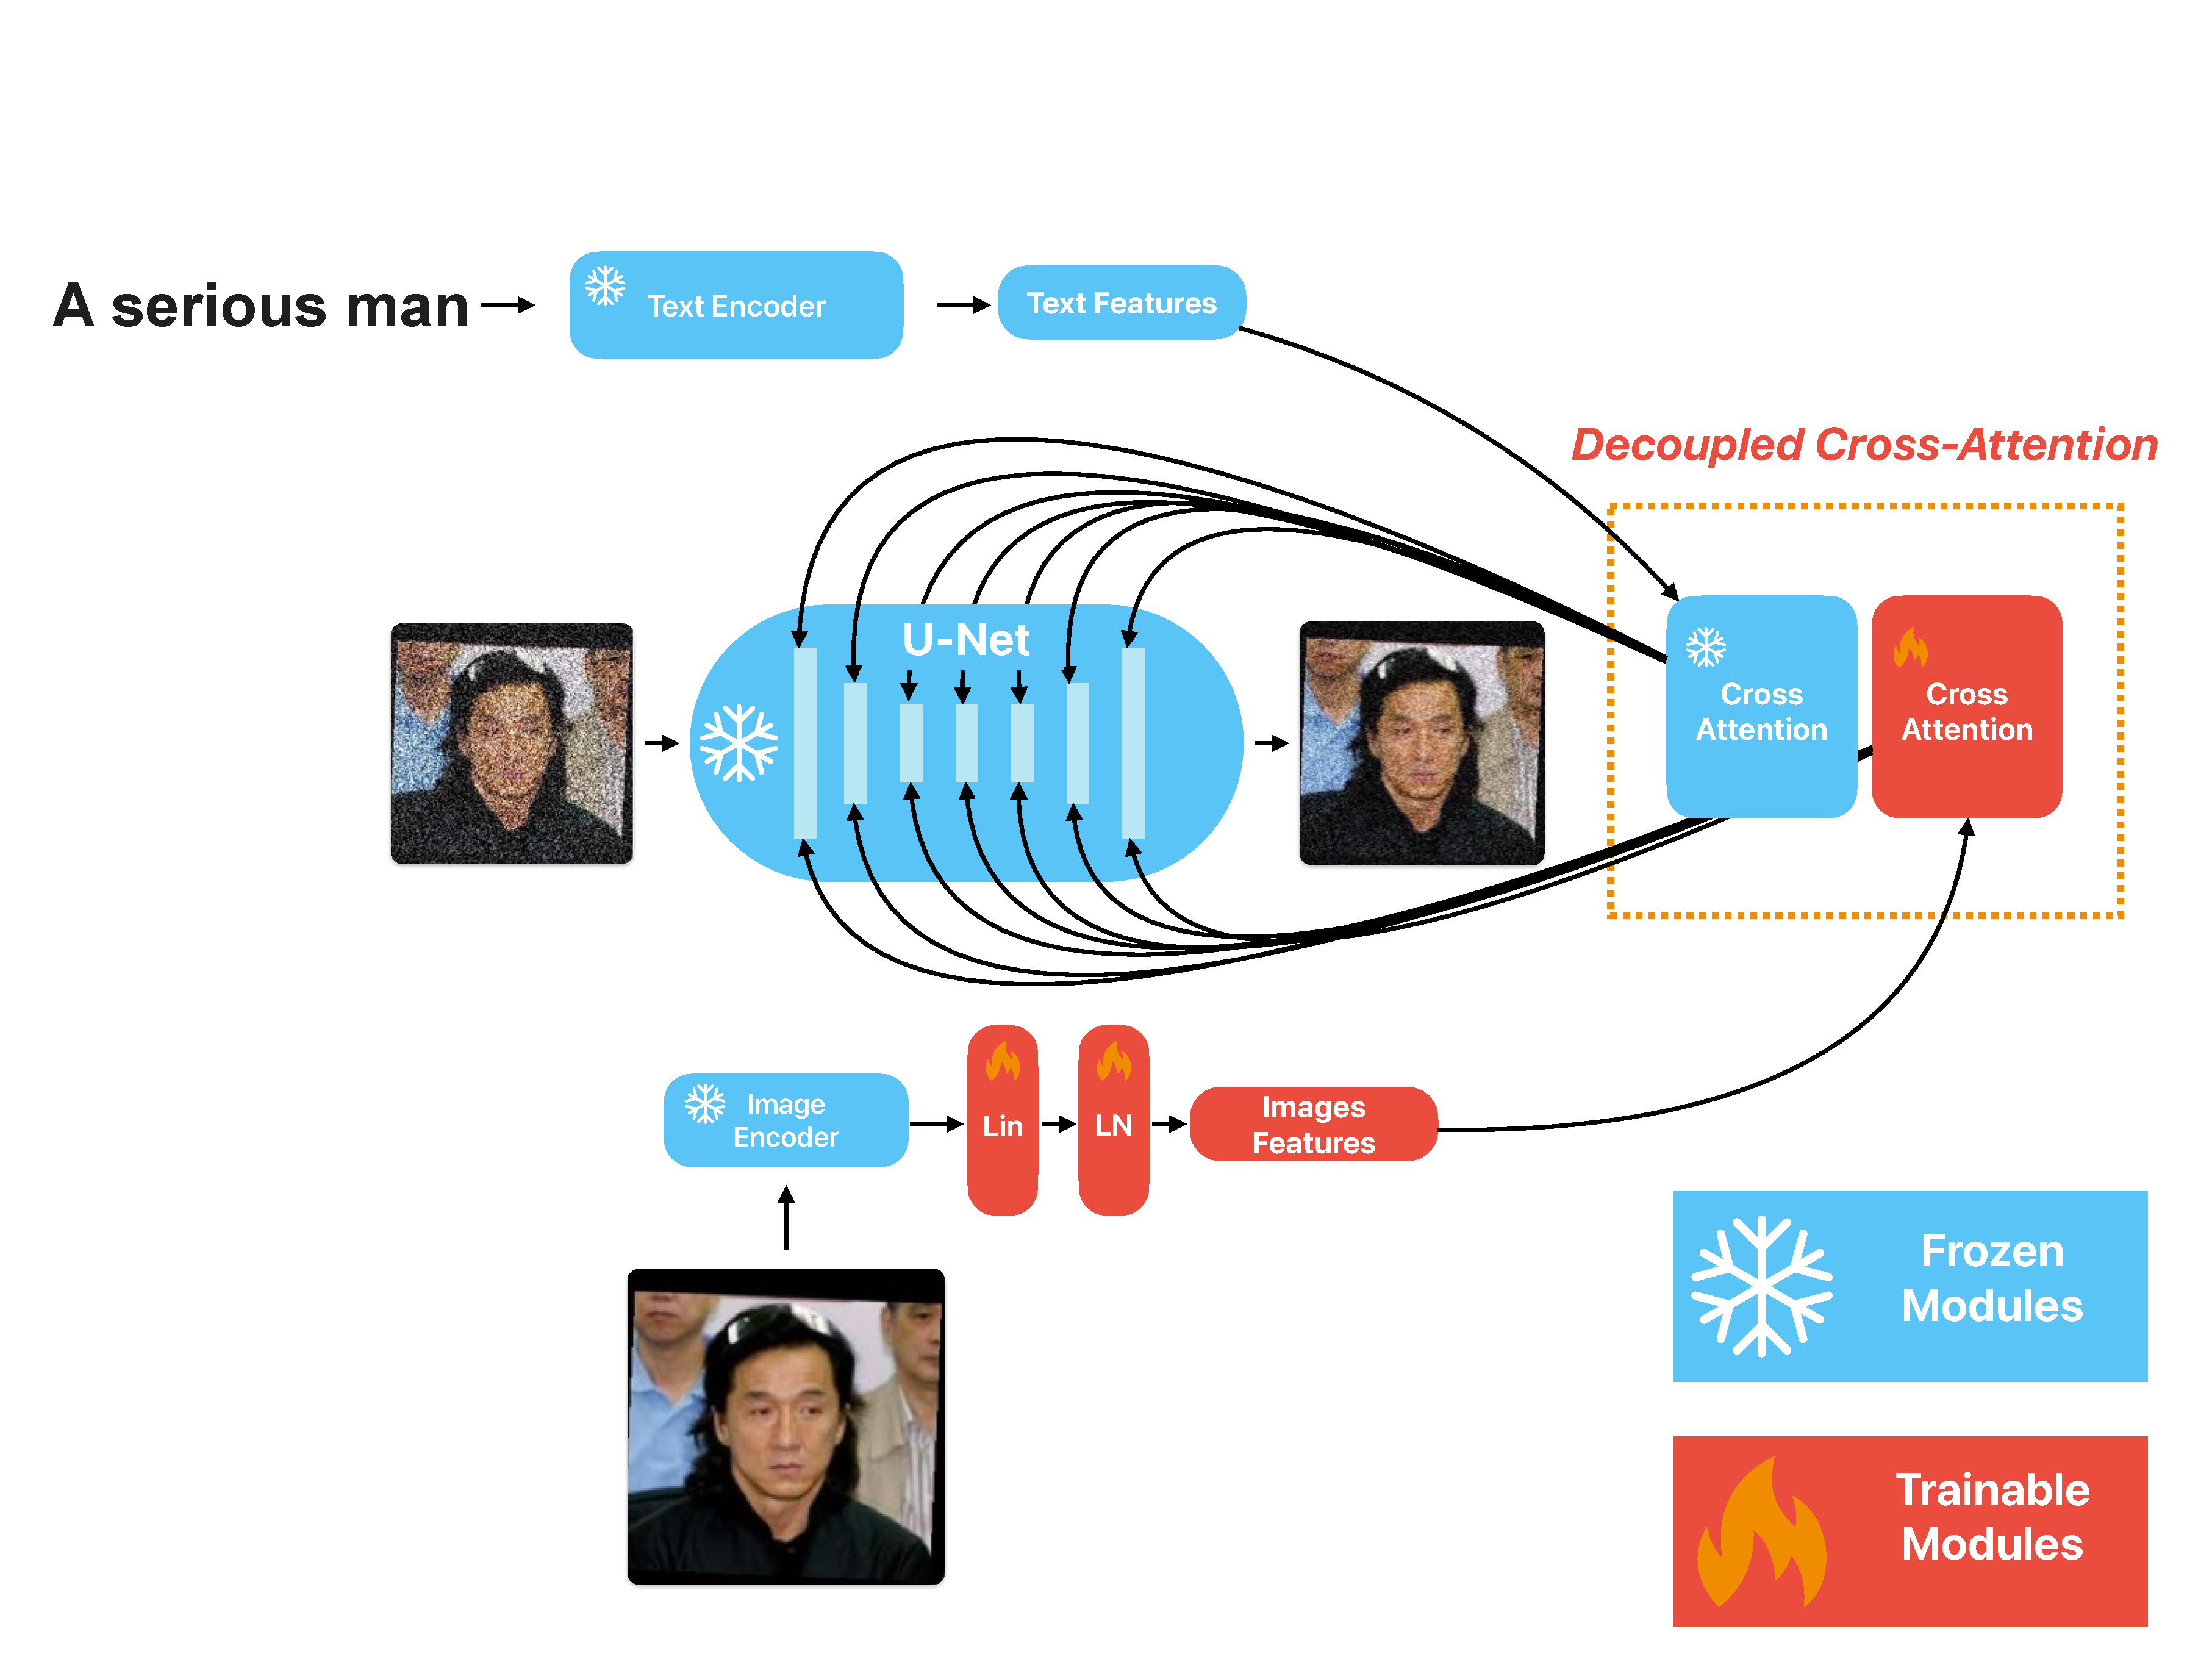
\includegraphics[width=1\textwidth]{ip-adapter.pdf}
    \caption{IP-Adapter}
    \label{fig:simple}
\end{figure}

IP-Adapter состоит из двух частей: image-энкодера для извлечения признаков изображения из промпта и адаптированных модулей с механизмом изолированного перекрестного внимания для встраивания признаков изображения в предобученную text-to-image модель.

Для получения признаков изображения используется обучаемая сеть, состоящая из линейного слоя и слоя нормализации, на вход которой подается эмбеддинг изображения, полученный с помощью предобученного image-энкодера CLIP. На этапе обучения вышеупомянутый энкодер заморожен.

Текстовые признаки, извлеченные из текстового энкодера CLIP, передаются в предобученную модель UNet через слои перекрестного внимания. Пусть даны признаки запроса $\mathbf{Z}$, признаки изображения $\mathbf{c_i}$ и текстовые признаки $\mathbf{c_t}$, тогда выход слоя перекрестного внимания $\mathbf{Z^{\prime}}$ определяется как: 
\begin{equation}
\mathbf{Z^{\prime}} = Attention(\mathbf{Q}, \mathbf{K}, \mathbf{V}) = softmax(\frac{\mathbf{QK^T}}{\sqrt{d}})\mathbf{V},
\end{equation}
где $\mathbf{Q} = \mathbf{ZW_q}, \mathbf{K} = \mathbf{c_t W_k}, \mathbf{V} = \mathbf{c_t W_v}$ --- матрицы запросов, ключей и значений механизма внимания для текстовых признаков соответственно, а $\mathbf{W_q, W_k, W_v}$ --- соответствующие матрицы весов. Для передачи в модель UNet признаков изображения каждому слою перекрестного внимания для текстовых признаков сопоставляется слой перекрестного внимания для признаков изображения. Пусть даны признаки изображения $c_i$, тогда выход нового слоя перекрестного внимания $\mathbf{Z^{\prime\prime}}$ определяется как: 
\begin{equation}
\mathbf{Z^{\prime\prime}} = Attention(\mathbf{Q, K^{\prime}, V^{\prime}}) = softmax(\frac{\mathbf{Q(K^{\prime})^T}}{\sqrt{d}})\mathbf{V^{\prime}},
\end{equation}
где $\mathbf{Q = Z W_q, K^{\prime} = c_i {W}^{\prime}_k, V^{\prime} = c_i {W}^{\prime}_v}$ --- матрицы запросов, ключей и значений механизма внимания для признаков изображения соответственно, а $\mathbf{{W}^{\prime}_k}$, $\mathbf{{W}^{\prime}_v}$ --- соответствующие матрицы весов. Выход изолированного перекрестного внимания получается как сумма вышеупомянутых выходов: 
\begin{equation}
\mathbf{Z^{new}} = softmax(\frac{\mathbf{QK^T}}{\sqrt{d}})\mathbf{V} +  softmax(\frac{\mathbf{Q(K^{\prime})^T}}{\sqrt{d}})\mathbf{V^{\prime}}
\end{equation}
Модель UNet замораживается, поэтому только $\mathbf{{W}^{\prime}_k}$ и $\mathbf{{W}^{\prime}_v}$ являются обучаемыми параметрами.

В процессе обучения минимизируется следующая функция потерь: 
\begin{equation}
\mathcal{L}(\epsilon, \epsilon_{\theta}) = \mathbb{E}_{\mathbf{x_t}, \epsilon, \mathbf{c_t}, \mathbf{c_i}, t} \|\epsilon - \epsilon_{\theta}(\mathbf{x_t}, \mathbf{c_t}, \mathbf{c_i}, t)\|^2,
\end{equation}
где $\mathbf{x_t}$ --- зашумленное изображение на шаге $t$.\par
Для того чтобы задействовать classifier-free guidance на этапе вывода, во время обучения случайным образом отбрасываются условия изображения: 
\begin{equation}
\hat{\epsilon}_{\theta}(\mathbf{x_t}, \mathbf{c_t}, \mathbf{c_i}, t) = w\epsilon_{\theta}(\mathbf{x_t}, \mathbf{c_t}, \mathbf{c_i}, t) + (1-w)\epsilon_{\theta}(\mathbf{x_t}, t)
\end{equation}

Если условие изображения отброшено, эмбеддинг соответствующего изображения зануляется. 

Поскольку перекрестное внимание к тексту и перекрестное внимание к изображению разделены, можно настроить вес условия изображения на этапе вывода: 
\begin{equation}
\mathbf{Z}^{new} = Attention(\mathbf{Q}, \mathbf{K}, \mathbf{V}) + \lambda \cdot Attention(\mathbf{Q}, \mathbf{K}^{\prime}, \mathbf{V}^{\prime}),
\end{equation}
где $\lambda$ --- весовой коэффициент. 

\subsection{IP-Adapter + агрегирующая функция}
\vspace{-45pt}
\begin{figure}[H]
    \centering
    \includegraphics[width=1\textwidth]{pooling.pdf}
    \caption{IP-Adapter + Pooling}
    \label{fig:pooling}
\end{figure}

Данный метод представляет собой модификацию метода IP-Adapter и принимает на вход несколько изображений вместо одного. К эмбеддингам входных изображений применяется агрегирующая функция (в нашем случае Max Pooling или Average Pooling)\cite{DBLP:journals/corr/abs-2009-07485}. Результат ее применения передается в полностью предобученный IP-Adapter.

\subsection{IP-Adapter + Self-Attention}
\vspace{-20pt}
\begin{figure}[h]
    \centering
    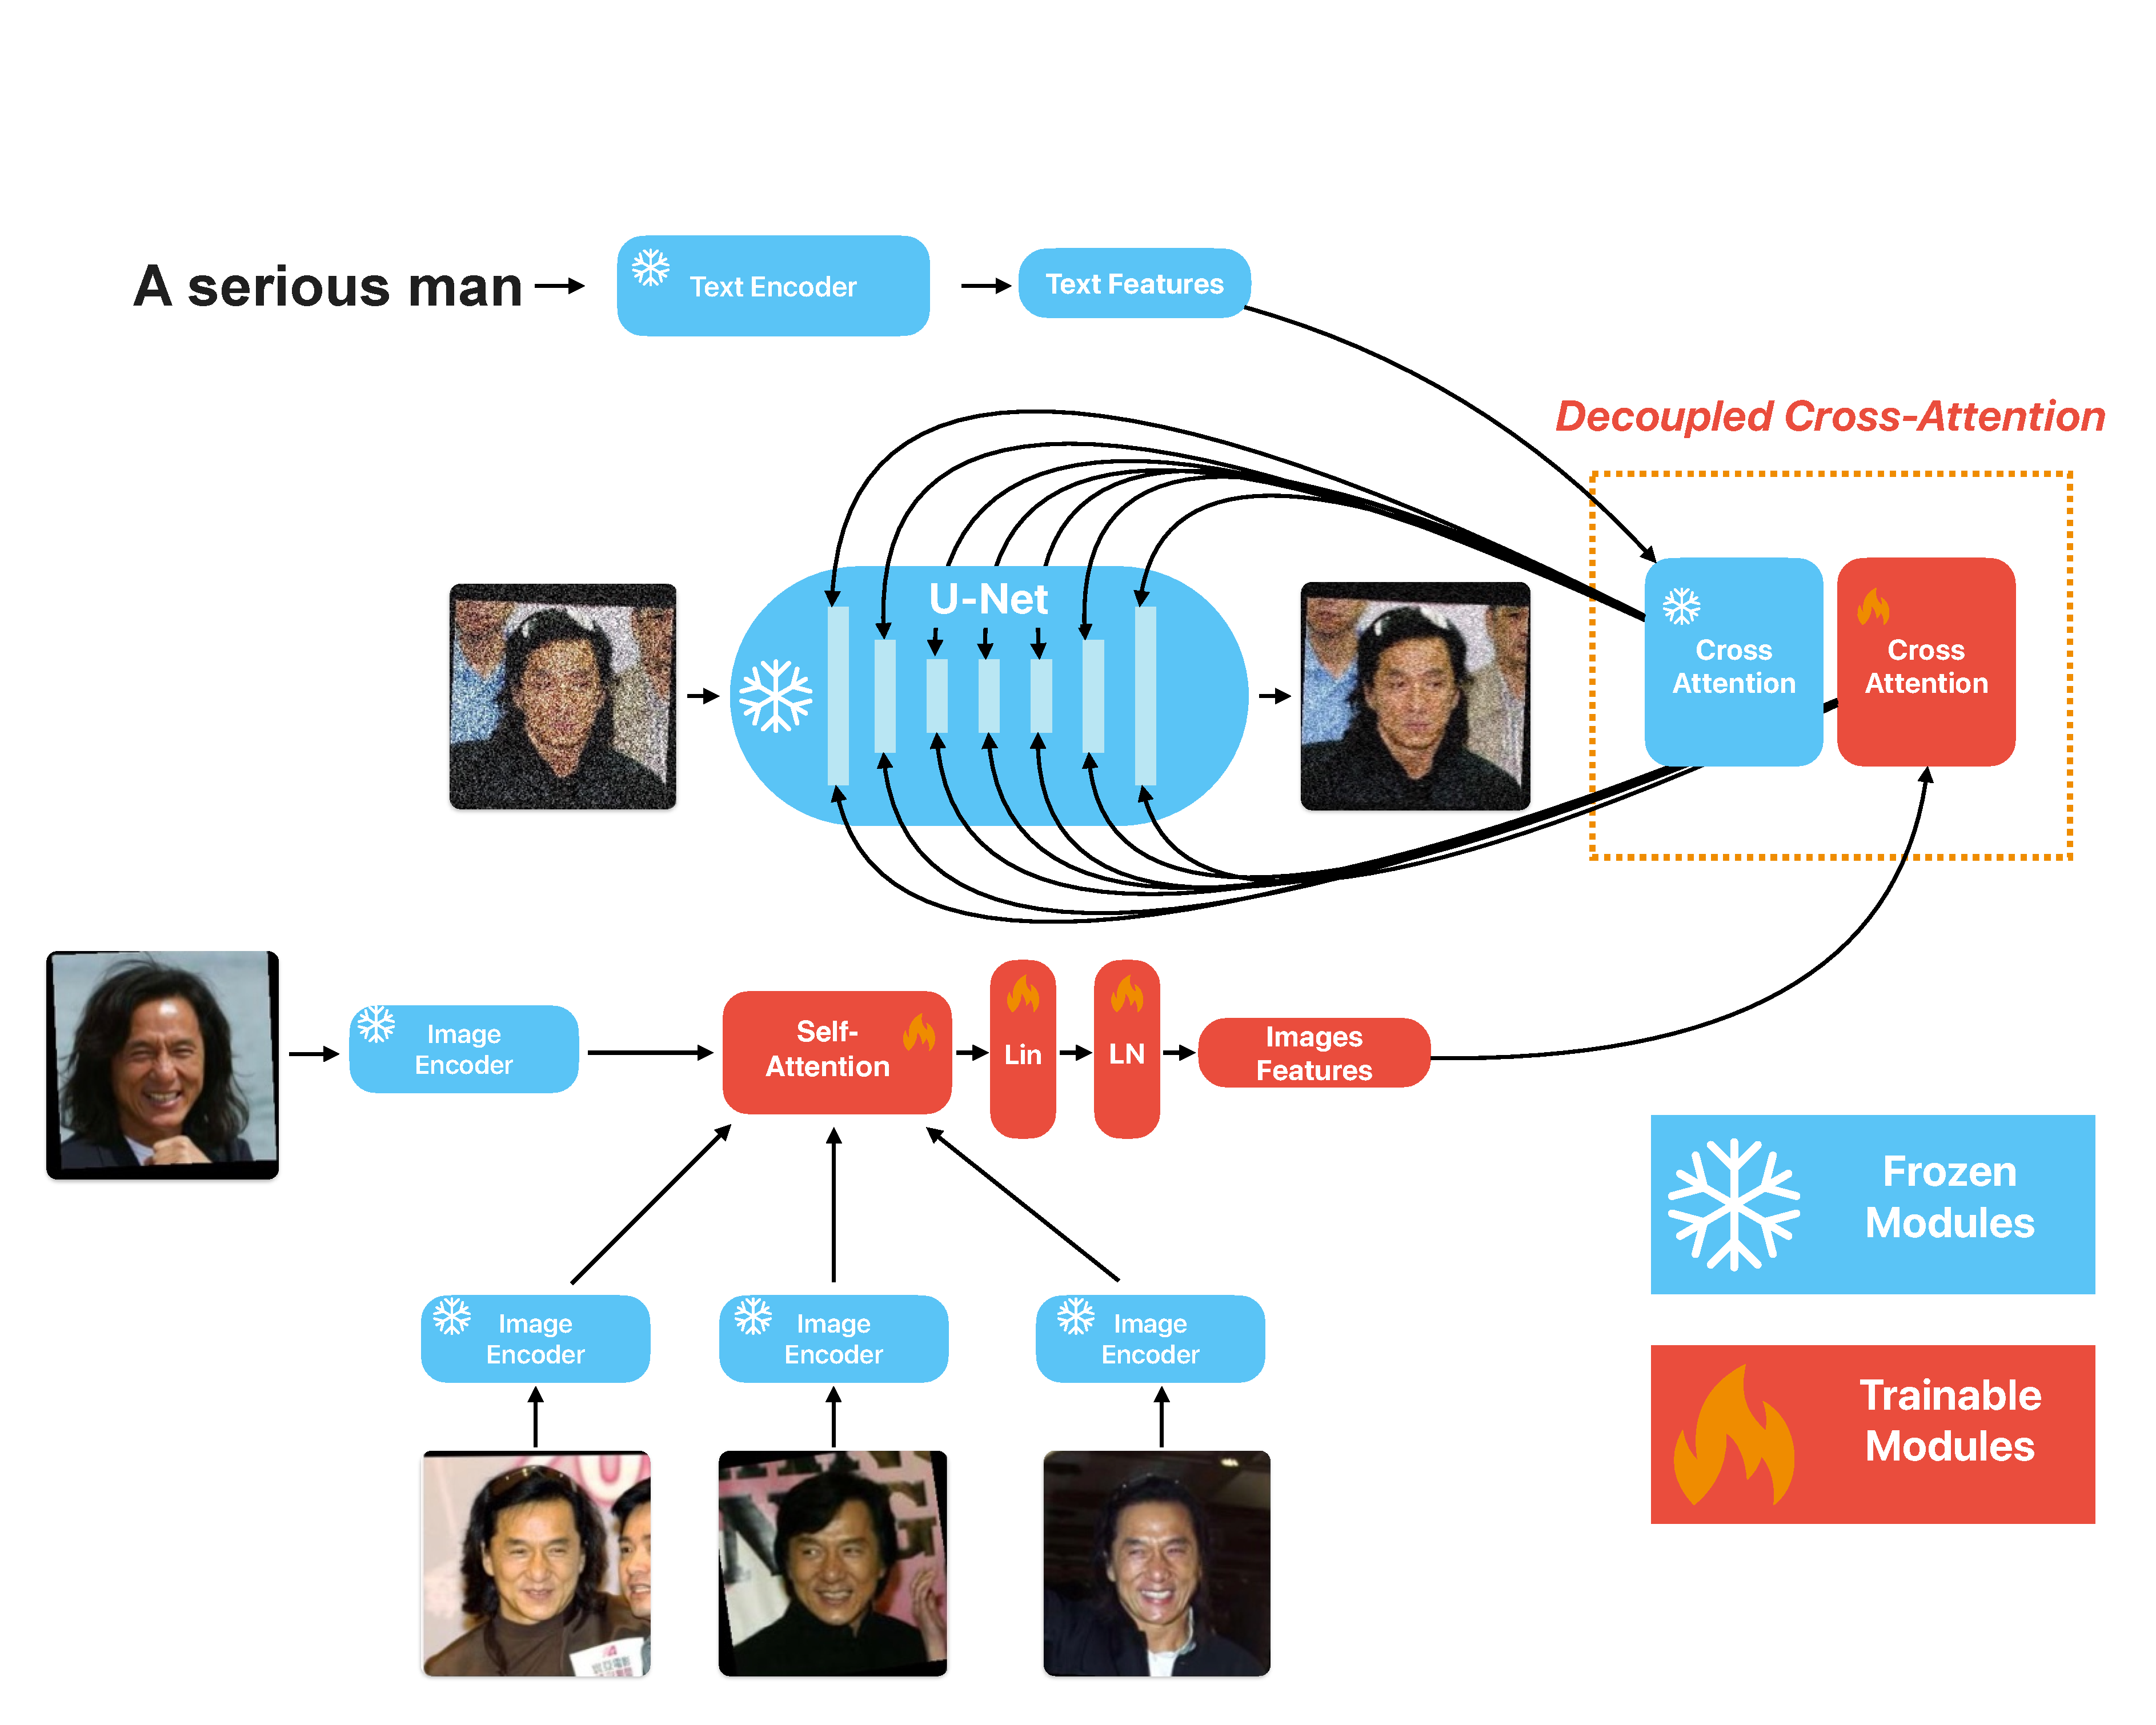
\includegraphics[width=1\textwidth]{self_attention.pdf}
    \caption{IP-Adapter + Self-Attention}
    \label{fig:self_attention}
\end{figure}

Предложенная модификация метода IP-Adapter включает в себя обработку нескольких изображений, к эмбеддингам которых применяется алгоритм Self-Attention\cite{DBLP:journals/corr/VaswaniSPUJGKP17}. На вход модели подается $N$ изображений одного объекта (в нашем случае $N = 10$), каждому из которых соответствует свой текстовый промпт. В ходе обучения случайным образом выбирается изображение, которое удаляется из рассмотрения, и модель пытается предсказать отброшенное изображение по его текстовому промпту и эмбеддингам оставшихся изображений, полученных с помощью image-энкодера CLIP.

\begin{algorithm}
\caption{Self-Attention}
\label{self_attention}
\begin{algorithmic}
\Procedure{Self-Attention}{$\mathbf{x}$}
    \State $\mathbf{Q} \gets \mathbf{x} \cdot \mathbf{W}_{q}$
    \State $\mathbf{K} \gets \mathbf{x} \cdot \mathbf{W}_{k}$
    \State $\mathbf{V} \gets \mathbf{x} \cdot \mathbf{W}_{v}$
    \State $\mathbf{Z} \gets \text{$softmax$}\left(\frac{\mathbf{Q} \cdot \mathbf{K}^T}{\sqrt{d}}\right) \cdot \mathbf{V}$
    \State \Return $\mathbf{Z}$
\EndProcedure
\end{algorithmic}
\end{algorithm}

После завершения работы модуля Self-Attention следуют модули IP-Adapter без изменений. В данном случае обучаемыми являются слои Self-Attention, Linear, Layer Norm и Cross-Attention. Поскольку модификация Self-Attention обучается на 9 изображениях, то, если на вход поступает большее или меньшее число изображений, в первом случае лишние изображения просто удаляются, а во втором запускается процедура бутстрепа до достижения нужного количества картинок.

\section{Вычислительный эксперимент}
Для экспериментов с вышеупомянутыми моделями используется датасет LFW Deep Funneled, который представляет собой набор изображений лиц людей вместе с их именами. В этом наборе данных 100 людям соответствует не меньше десяти разных фотографий. 

\begin{figure}[H]
\begin{minipage}{.25\textwidth}
    \centering
    \includegraphics[width=1\textwidth]{Catherine_Zeta-Jones_0004.jpg}
    \label{fig:1}
\end{minipage}%
\begin{minipage}{.25\textwidth}
    \centering
    \includegraphics[width=1\textwidth]{Catherine_Zeta-Jones_0006.jpg}
    \label{fig:2}
\end{minipage}%
\begin{minipage}{.25\textwidth}
    \centering
    \includegraphics[width=1\textwidth]{Catherine_Zeta-Jones_0008.jpg}
    \label{fig:3}
\end{minipage}%
\begin{minipage}{.25\textwidth}
    \centering
    \includegraphics[width=1\textwidth]{Catherine_Zeta-Jones_0010.jpg}
    \label{fig:4}
\end{minipage}%
\vspace{-12pt}
\begin{minipage}{.25\textwidth}
    \centering
    \includegraphics[width=1\textwidth]{Tom_Hanks_0002.jpg}
    \label{fig:11}
\end{minipage}%
\begin{minipage}{.25\textwidth}
    \centering
    \includegraphics[width=1\textwidth]{Tom_Hanks_0005.jpg}
    \label{fig:21}
\end{minipage}%
\begin{minipage}{.25\textwidth}
    \centering
    \includegraphics[width=1\textwidth]{Tom_Hanks_0008.jpg}
    \label{fig:31}
\end{minipage}%
\begin{minipage}{.25\textwidth}
    \centering
    \includegraphics[width=1\textwidth]{Tom_Hanks_0009.jpg}
    \label{fig:41}
\end{minipage}%
\caption{Примеры изображений из датасета LFW Deep Funneled.}
\end{figure}

Исходный датасет разделяется на тренировочную и тестовую выборки в соотношении $2:1$. Модель IP-Adapter + Self-Attention обучается на тренировочной выборке, содержащей набор персон, каждой из которых соответствует имя персоны и несколько её изображений.  Процесс обучения описан выше. В остальных случаях для генерации используются предобученные модели, процедура дообучения не проводится. 

\begin{figure}[H]
\begin{figure}[H]
\begin{minipage}{.25\textwidth}
    \centering
    DreamBooth
    \label{fig:dm0}
\end{minipage}%
\begin{minipage}{.25\textwidth}
    \centering
    \includegraphics[width=0.9\textwidth]{dm1.jpeg}
    \label{fig:dm1}
\end{minipage}%
\begin{minipage}{.25\textwidth}
    \centering
    \includegraphics[width=0.9\textwidth]{dm2.jpeg}
    \label{fig:dm2}
\end{minipage}%
\begin{minipage}{.25\textwidth}
    \centering
    \includegraphics[width=0.9\textwidth]{dm3.jpeg}
    \label{fig:dm3}
\end{minipage}%
\end{figure}

\vspace{-25pt}

\begin{figure}[H]
\begin{minipage}{.25\textwidth}
    \centering
    IP-Adapter
    \label{fig:ip0}
\end{minipage}%
\begin{minipage}{.25\textwidth}
    \centering
    \includegraphics[width=0.9\textwidth]{ip1.jpeg}
    \label{fig:ip1}
\end{minipage}%
\begin{minipage}{.25\textwidth}
    \centering
    \includegraphics[width=0.9\textwidth]{ip2.jpeg}
    \label{fig:ip2}
\end{minipage}%
\begin{minipage}{.25\textwidth}
    \centering
    \includegraphics[width=0.9\textwidth]{ip3.jpeg}
    \label{fig:ip3}
\end{minipage}%
\end{figure}

\vspace{-25pt}

\begin{figure}[H]
\begin{minipage}{.25\textwidth}
    \centering
    IP-Adapter + Max Pooling
    \label{fig:mp0}
\end{minipage}%
\begin{minipage}{.25\textwidth}
    \centering
    \includegraphics[width=0.9\textwidth]{mp1.png}
    \label{fig:mp1}
\end{minipage}%
\begin{minipage}{.25\textwidth}
    \centering
    \includegraphics[width=0.9\textwidth]{mp2.png}
    \label{fig:mp2}
\end{minipage}%
\begin{minipage}{.25\textwidth}
    \centering
    \includegraphics[width=0.9\textwidth]{mp3.png}
    \label{fig:mp3}
\end{minipage}%
\end{figure}

\vspace{-25pt}

\begin{figure}[H]
\begin{minipage}{.25\textwidth}
    \centering
    IP-Adapter + Avg Pooling
    \label{fig:mp0}
\end{minipage}%
\begin{minipage}{.25\textwidth}
    \centering
    \includegraphics[width=0.9\textwidth]{ap1.jpeg}
    \label{fig:ap1}
\end{minipage}%
\begin{minipage}{.25\textwidth}
    \centering
    \includegraphics[width=0.9\textwidth]{ap2.jpeg}
    \label{fig:ap2}
\end{minipage}%
\begin{minipage}{.25\textwidth}
    \centering
    \includegraphics[width=0.9\textwidth]{ap3.jpeg}
    \label{fig:ap3}
\end{minipage}%
\end{figure}

\vspace{-25pt}

\begin{figure}[H]
\begin{minipage}{.25\textwidth}
    \centering
    IP-Adapter + Self-Attention
    \label{fig:sa0}
\end{minipage}%
\begin{minipage}{.25\textwidth}
    \centering
    \includegraphics[width=0.9\textwidth]{sa1.jpeg}
    \label{fig:sa1}
\end{minipage}%
\begin{minipage}{.25\textwidth}
    \centering
    \includegraphics[width=0.9\textwidth]{sa2.jpeg}
    \label{fig:sa2}
\end{minipage}%
\begin{minipage}{.25\textwidth}
    \centering
    \includegraphics[width=0.9\textwidth]{sa3.jpeg}
    \label{fig:sa3}
\end{minipage}%
\end{figure}
\caption{Результаты генерации для рассмотренных моделей.}
\end{figure}

Точность качества генерации оценивается по метрикам Frechet Inception Distance (FID) и Inception Score (IS). Результаты приведены в таблице: 

\begin{table}[H]
\begin{tabular}{l c c c c}
\toprule
\textbf{Метод} & \textbf{IS} \textuparrow & \textbf{FID} \textdownarrow \\
\midrule
IP-Adapter & 15.37  & 8.92\\
DreamBooth & 17.64 & 9.61\\
IP-Adapter + Max Pooling & 14.12 & 10.10\\
IP-Adapter + Avg Pooling & 13.56 & 11.82\\
IP-Adapter + Self-Attention & $\mathbf{18.72}$ & $\mathbf{7.56}$\\
\bottomrule
\end{tabular}
\vspace{8pt}
\caption{Сравнение предлагаемых нами методов с существующими по метрикам IS и FID на датасете LFW Deep Funneled. Лучшие результаты выделены жирным шрифтом.}
\end{table}

\section{Заключение}
Модели генерации текста в изображение подтолкнули вперед возможности искусственного интеллекта, позволяя создавать качественные и разнообразные изображения на основе текстовых описаний. Тем не менее, возникают трудности при создании изображений конкретных объектов, таких как люди, из-за ограничений точности и передачи идентичности. Для преодоления этих проблем мы предложили новые решения, в том числе улучшенная модификация IP-Адаптера, которая умеет обрабатывать несколько изображений одновременно и улучшает качество генерации. В качестве агрегирующей функции были рассмотрены Pooling и механизм Self-Attention. Данные методы показали высокие значения на метриках качества FID и IS. В дальнейшем существует возможность модифировать уже наши алгоритмы посредством использования LoRA\cite{DBLP:journals/corr/abs-2106-09685}, FaceNet\cite{DBLP:journals/corr/SchroffKP15}  и других.


\bibliographystyle{plain}
\bibliography{references}

\end{document}
